\documentclass[final]{cmpreport}
\usepackage{natbib}
\usepackage{graphicx}
\usepackage{wrapfig}
\usepackage{paralist}
\usepackage{outlines}
\usepackage{booktabs}
\usepackage{appendix}
\usepackage{float}
\usepackage{algorithm}
\usepackage{algpseudocode} % http://ctan.org/pkg/algorithm
\usepackage{wrapfig}
\graphicspath{ {./} }

\renewcommand{\algorithmicrequire}{\textbf{Input:}}
\renewcommand{\algorithmicensure}{\textbf{Output:}}

\definecolor{light-gray}{gray}{0.95}
\newcommand{\code}[1]{\colorbox{light-gray}{\texttt{#1}}}

\title{Third Year Project: Report}
\author{Matthew Taylor}
\registration{100151729}
\supervisor{Dr Rudy Lapeer}
\ccode{CMP-6013Y}

\summary{This report details an implementation of procedural generation in a video game environment.}

\acknowledgements{I would like to thank Dr Rudy Lapeer, from University of East Anglia, for his wisdom and guidance.}

\begin{document}

\maketitle

\begin{section}{Introduction}

\subsection{Aim of the project}
The project aimed to implement a first person video game which uses procedural generation to provide a novel and interesting game experience. The project will explore the technical aspects of using PCG as a core feature of a game, specifically, implementation and performance. 

\subsection{Motivation}
Procedural generation is not a new field, especially in video games, but there are interesting areas that are seldom explored. One of these areas is real-time procedural generation.

The motivation behind the project's aims were to explore new and interesting concepts, namely, using PCG as a core feature in a game and using real-time procedural generation to provide an interesting experience.

\subsection{Literature}
The project also drew inspiration and guidance from existing PCG games, as described in papers by \citet{spufford_2003}, \cite{welsh_2016} and \cite{gct-spelunky}.

The project also took into account the wealth of research done on PCG techniques, as described in papers by \cite{Perlin:1985:IS:325165.325247}, \cite{ebert2003texturing} and \cite{Dormans:2010:ALD:1814256.1814257}.
   

\end{section}

\begin{section}{Design and planning}

\subsection{Implementation methodology}
The project development operated under an Agile methology. Agile does not require that all requirements (or ``user stories'') are defined up front, instead it is encouraged that they are developed and refined during the lifecycle of the project.

The project itself was divided into Agile ``sprints''. It was decided to deliver a sprint every two weeks, as this fit with the development time given to the project and providing updates to the project supervisor.

While all the stories were not required at the outset, as part of the planning, it was decided to plot rough timescales against Agile ``epics''. These epics provide a high-level view of functionality and are detailed in Table \ref{tab:epics} in Appendix D.

The epics also contain very high-level user stories, which provide a little more detail. These were decided at the project outset, then refined during development. Before any user story can be developed, it was required that more detailed requirements were written. These were then recorded and tracked on Trello. 

\subsection{Implementation plan}

With the high-level design documented in the epics, planning of these epics against timescales was required. This timeline plan is visible in Figure \ref{fig:gantt1} in Appendix A. Progress was then tracked against this Gantt chart to ensure that progress was being made and that the project could be achieved as planned.

As the project was run using Agile principles, the Gantt chart was revised to reflect changes to the plan. These changes are visible in Figure \ref{fig:gantt2} in Appendix A. 

Changes to the Gantt chart include the addition of a Level Generation task - the Level Re-Generator. This reflects a focus of the project on procedurally re-generating levels in real-time, so this has been split out as a seperate task and given a shorter timescale, reflecting the importance of the task to the project.

The gameplay section was split into two tasks, reflecting the focus on implementing core gameplay as a priority, with enhanced gameplay being desirable but not as critical to the evaluation of success of the project.

\subsection{UML}

As the project began, a UML diagram was designed to provide a high level framework to work towards. Unity does not prescribe much structure, so a UML design to begin with was useful. The initial UML design can be seen in Figure \ref{fig:uml1} in Appendix B. The iterated design can be seen in Figure \ref{fig:uml2} in Appendix B, which shows the definition of classes being enhanced with the additional methods and attributes required to support the design, as well as the addition of the \textbf{Level Re-Generator} class.


\subsection{Requirements and prioritisation}

The project defined epics (or, high level requirements) at the outset, with more detailed requirements written at each stage. This allows the project the be flexible, with lessons learned in the prototyping incorporated into future requirements. It also saves time, because requirements do not need to be written in advance when they would likely be changed anyway.

The epics and requirements written for the project so far are available in the appendix in Table \ref{tab:epicreqs} on \pageref{tab:epicreqs}.


\subsection{Design prototypes}
\subsubsection{Guaranteed path generation}
The first part of the design to be implemented required a guaranteed path through a maze to be generated. This was achieved by using a random walk - a stochastic process implmented in two dimensions to provide a definite route through the maze.

The random walk is implemented using an agent based approach. The agent can choose from three random directions to travel in - left, right or down. These probabilities are detailed in Table \ref{tab:probdirs}. When the agent has chosen a valid direction, it randomly selects a valid tile. 

The agent has methods of checking where it has been and where it is going next, so that it picks valid tiles that have openings in the directions it has come from and intends to go. The agent is given bounds and restrictions while it is performing the random walk, which provides a method of parameterising the level and deciding on an endpoint. 

\subsubsection{Decoration of rooms}

Rooms are decorated with interior sub-dividing walls and other elements to provide a convincing and interesting environment to traverse. Decoration is achieved by populating each room with a random pre-defined set of geometry, examples of which can be seen in Figures \ref{fig:prefab-room}, \ref{fig:prefab-int} and \ref{fig:room}, in Appendix C. 

In the prototype design, a single point is used to populate all geometry from the centre of the room. However, iterations on the design will use several points which an agent will scan through to populate things like sub-rooms, corridors, walls and desks with appropriate decorations, providing considerable variation for little asset generation cost.

\subsection{Evaluation of success} \label{evalsuccess}
A key issue with this project is evaluating if it is successful. If there is no clear notion of what success looks like, the project could progress in unproductive directions. Below are the key measures of success chosen at the start of the project to measure success against.

\subsubsection{Convincing levels}
The levels must appear convincing. This is difficult to quantify, but nevertheless is an important attribute. The levels (at least in the initial design) will be mazes generated in a grid, with the grid sections subdivided in different ways.

This could easily create a boring level, where the grid pattern is discernable and the rooms are boring and procedural to traverse. Successful generation of levels will avoid these issues.

\subsubsection{Convincing decoration}
The decoration in each individual room will contribute to how convincing and hand-crafted each level looks. As described in \cite{doi:10.1111/j.1467-8659.2009.01351.x} and \cite{taylor-parberry}, there are several challenges to making room decoration appear to be hand-made when it is procedurally generated. Of particular focus will be generating furniture and objects in positions that feel realistic and unique.

\subsubsection{Performance}
Performance is another key component of the project succeeding. If the game responds poorly, it will be frustrating to play. Performance will be measured in a few ways:
\begin{compactitem}
    \item{\textbf{Framerate}: must be at least 30 frames per second}
    \item{\textbf{Initial loading time}: must take less than 30 seconds}
    \item{\textbf{Smooth level re-generation}: no dip in framerate below 30 frames per second}
\end{compactitem}

\subsection{Experimental methodology}
The experimental results of the project will focus entirely on performance, as this is objectively measureable, as compared to the more subjective nature of how convincing the levels are. The experiments will focus on two main areas of performance: generation time performance and runtime performance.

\subsubsection{Generation time performance}
The experiments around the time it takes to procedurally generate levels will be simple timing experiments, using Unity scripting methods to provide timings of the time it takes to generate levels. These experiments will be run multiple times, with averages taken, to provide more accurate results.

The experiments will be run on different parameters, like level size, to test how effective the procedural generation implementation is at scale.

\subsubsection{Runtime performance}
Runtime performance will be evaluated using the Unity Profiler tool. This (by default) provides a detailed snapshot of system resources and performance metrics from a rolling 300ms window of gameplay. For the experiments, the game will be allowed to generate the level and when gameplay begins, a 5 second period of movement will be allowed to elapse before measurements are taken. This is to allow for the performance to stabilise. These experiments will be repeated multiple times, with averages taken, to provide more accurate results.

These experiments will be run on several different parameters, comparing:

\begin{compactitem}
    \item{Different map sizes}
    \item{Static vs real-time map regeneration}
    \item{Whether AIs are navigating the level}
    \item{Whether map culling is enabled}
\end{compactitem}

Performance tests were run using the Unity Editor, as compared to compiled version of the code. This was done for two reasons, the first being that much of the timing experiment code outputs to a debug console. The second reason is that the Unity Editor is required to use the Unity Profiler (see \citet{technologies_2019}) in order to access detailed performance statistics.

\subsubsection{Reference hardware}
To ensure consistent results, the same hardware was used for all experiments and a consistent test environment was established. The hardware used for testing was considered to be a reasonable reflection of recent PC hardware - it is not sufficiently powerful to make the results unreplicable by other users.

The reference hardware specification was:
\begin{compactitem}
    \item{\textbf{Operating System}: Windows 10 Home}
    \item{\textbf{CPU}: Intel Core i5-7200 @ 2.5GHz}
    \item{\textbf{Graphics}: Intel HD Graphics 620 (integrated chipset)}
    \item{\textbf{RAM}: 8GB}
\end{compactitem}

The test environment involved running Windows 10 with no other applications open, except for the Unity Editor. All tests were run operating on mains power, so no power-saving CPU throttling would occur. 

\end{section}

\begin{section}{Implementation}
- Screenshots of game working
- Commented code
- Technical documentation

\end{section}

\begin{section}{Evaluation}

\subsection{Quality of levels}
- Write about the quality of my levels

\subsection{Level generation performance}
Experiments were run to evaluate the performance of the level generation algorithm. The first experiment involved timing code being added to the level generation code, as detailed in Algorithm \ref{algo1}.

\subsubsection{Generation code execution testing}

\begin{algorithm}[H]
    \caption{Level Generation Timing Code}
    \label{algo1}
    \begin{algorithmic}[1]
        \Require Level Generation Size ${S}$
        \Ensure Time Elapsed $T$
        \State{{$t \leftarrow Start Time$}} \Comment{{\em set the time the generation started}}
        \State{Initialise}
        \State{Place all tile spawn points} \Comment{{\em based on $S$}}
        \State{Generate Critical Path} \Comment{{\em adds rooms/interiors with guaranteed route to goal}}
        \For{$i \leftarrow 1$ to $S$} \Comment{{\em for each tile wide}}
        \For{$j \leftarrow 1$ to $S$} \Comment{{\em for each tile deep}}
            \If{$Tile not generated$} \Comment{{\em check tile not on critical path}}
                \State{Add filler tiles} \Comment{{\em add random tile}}
                \State{Add room interiors} \Comment{{\em adds random interior}}
                \State{Add doors} \Comment{{\em adds random doors}}
            \EndIf{}
        \EndFor{}
        \EndFor{}

        \State{return $T \leftarrow time now - t$ \Comment{{\em return time elapsed}}}

\end{algorithmic}
\end{algorithm}

Varying sizes of level generation grids were used and each experiment run multiple times to provide averaged results. The generation times are displayed in Table \ref{tab:genres1}.

\begin{wraptable}{R}{0.5\textwidth}

    \centering
    \resizebox{0.49\textwidth}{!}{%
    \begin{tabular}{|l|l|l|}
    \hline
    \textbf{\begin{tabular}[c]{@{}l@{}}Level Size\\ (in tiles)\end{tabular}} & \textbf{Number of tiles} & \textbf{\begin{tabular}[c]{@{}l@{}}Generation Time\\ (in seconds)\end{tabular}} \\ \hline
    3x3 & 9 & 0.630 \\
    5x5 & 25 & 0.790 \\
    7x7 & 49 & 0.591 \\
    9x9 & 81 & 0.665 \\
    10x10 & 100 & 0.937 \\
    12x12 & 144 & 0.929 \\
    15x15 & 225 & 0.914 \\
    18x18 & 324 & 0.921 \\
    20x20 & 400 & 0.953 \\ \hline
    \end{tabular}%
    }
    \caption{Timing results from timing the level generation code of varying size of levels}
    \label{tab:genres1}

\end{wraptable}

These results demonstrate that the time taken to run the level generation script does not scale significantly with increasing the level size. However, from running the tests it was clear generating a large level (eg, 10x10 or bigger) was taking longer than the reported time of less than a second. It was observed that from starting the game to being able to play it was taking several seconds longer than this.

\subsubsection{Profiling the generation code}
It was clear from the experiments that even though the generation code runs quickly, even with large levels, the time taken to having a playable level took longer. A new experiment was devised, using the Unity Profiler to gather more accurate and usable results.

\begin{wrapfigure}{R!}{0.5\textwidth}
    \centering
    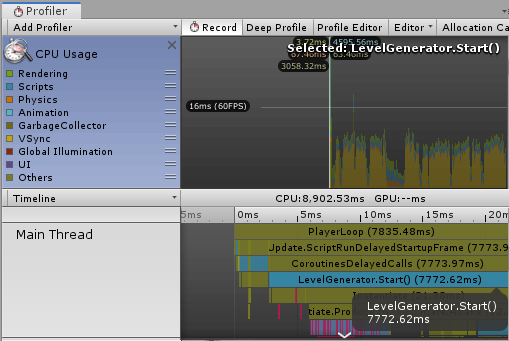
\includegraphics[width=0.49\textwidth]{img/Profiler10x10.png}
    \caption{Unity Profiler showing execution time of LevelGenerator script}
    \label{fig:profiler}
\end{wrapfigure}

The Unity Profiler incurs additional overhead from being used, however the overhead is consistent so results are still useful. The Profiler provides very detailed information, but for this experiment only one measure was considered - the time to run the LevelGenerator script during the first frame of execution. An screenshot of the Unity Profiler show results from the first frame can be seen in Figure \ref{fig:profiler}.

The Profiler provides more accurate data, because it measures the time taken to load geometry and textures onto the GPU. This explains the gap between the initial experiment and the observed results, because for large levels a significant amount of level geometry is required to be loaded.

% Please add the following required packages to your document preamble:
% \usepackage{graphicx}
\begin{table}[]
    \centering
    \begin{tabular}{|l|l|l|}
    \hline
    \textbf{\begin{tabular}[c]{@{}l@{}}Level Size\\ (in tiles)\end{tabular}} & \textbf{Number of tiles} & \textbf{\begin{tabular}[c]{@{}l@{}}Profiled Generation\\ Time (in seconds)\end{tabular}} \\ \hline
    3x3 & 9 & 0.595 \\
    5x5 & 25 & 1.974 \\
    7x7 & 49 & 2.965 \\
    9x9 & 81 & 5.842 \\
    10x10 & 100 & 6.754 \\
    12x12 & 144 & 12.516 \\
    15x15 & 225 & 25.183 \\
    18x18 & 324 & 53.932 \\
    20x20 & 400 & 86.276 \\ \hline
    \end{tabular}%
    \caption{Timing results from profiling the level generation script execution of varying size of levels}
    \label{tab:genres2}
\end{table}

The results of the profiling are shown in Table \ref{tab:genres2}. They are much more realistic when compared to anecdotal evidence of observing the performance of the game.

\begin{wrapfigure}{L!}{0.5\textwidth}
    \centering
    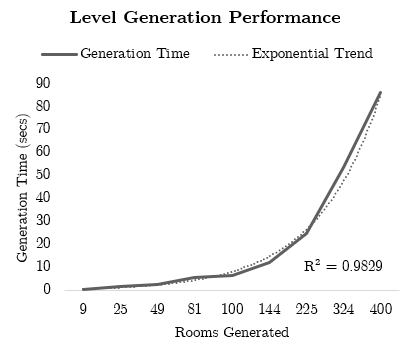
\includegraphics[width=0.49\textwidth]{img/genperftable.png}
    \caption{Results of profiled generation performance}
    \label{fig:genperftable}
\end{wrapfigure}

When plotted on a graph, as shown in Figure \ref{fig:genperftable}, the relationship between the number of rooms generated and the generation time can be seen. It was hypothesised that as the number of rooms increases exponentially, because it is based on a grid of $n x n$ dimensions, that the generation time would also increase exponentially. The plotted trendline and the high $R^2$ value demonstrates this. 

\subsection{In-game performance evaluation}



\end{section}



\bibliography{sources}

\newpage

\appendix

\begin{section}{Gantt charts}

\begin{figure}[H]
    \centering
    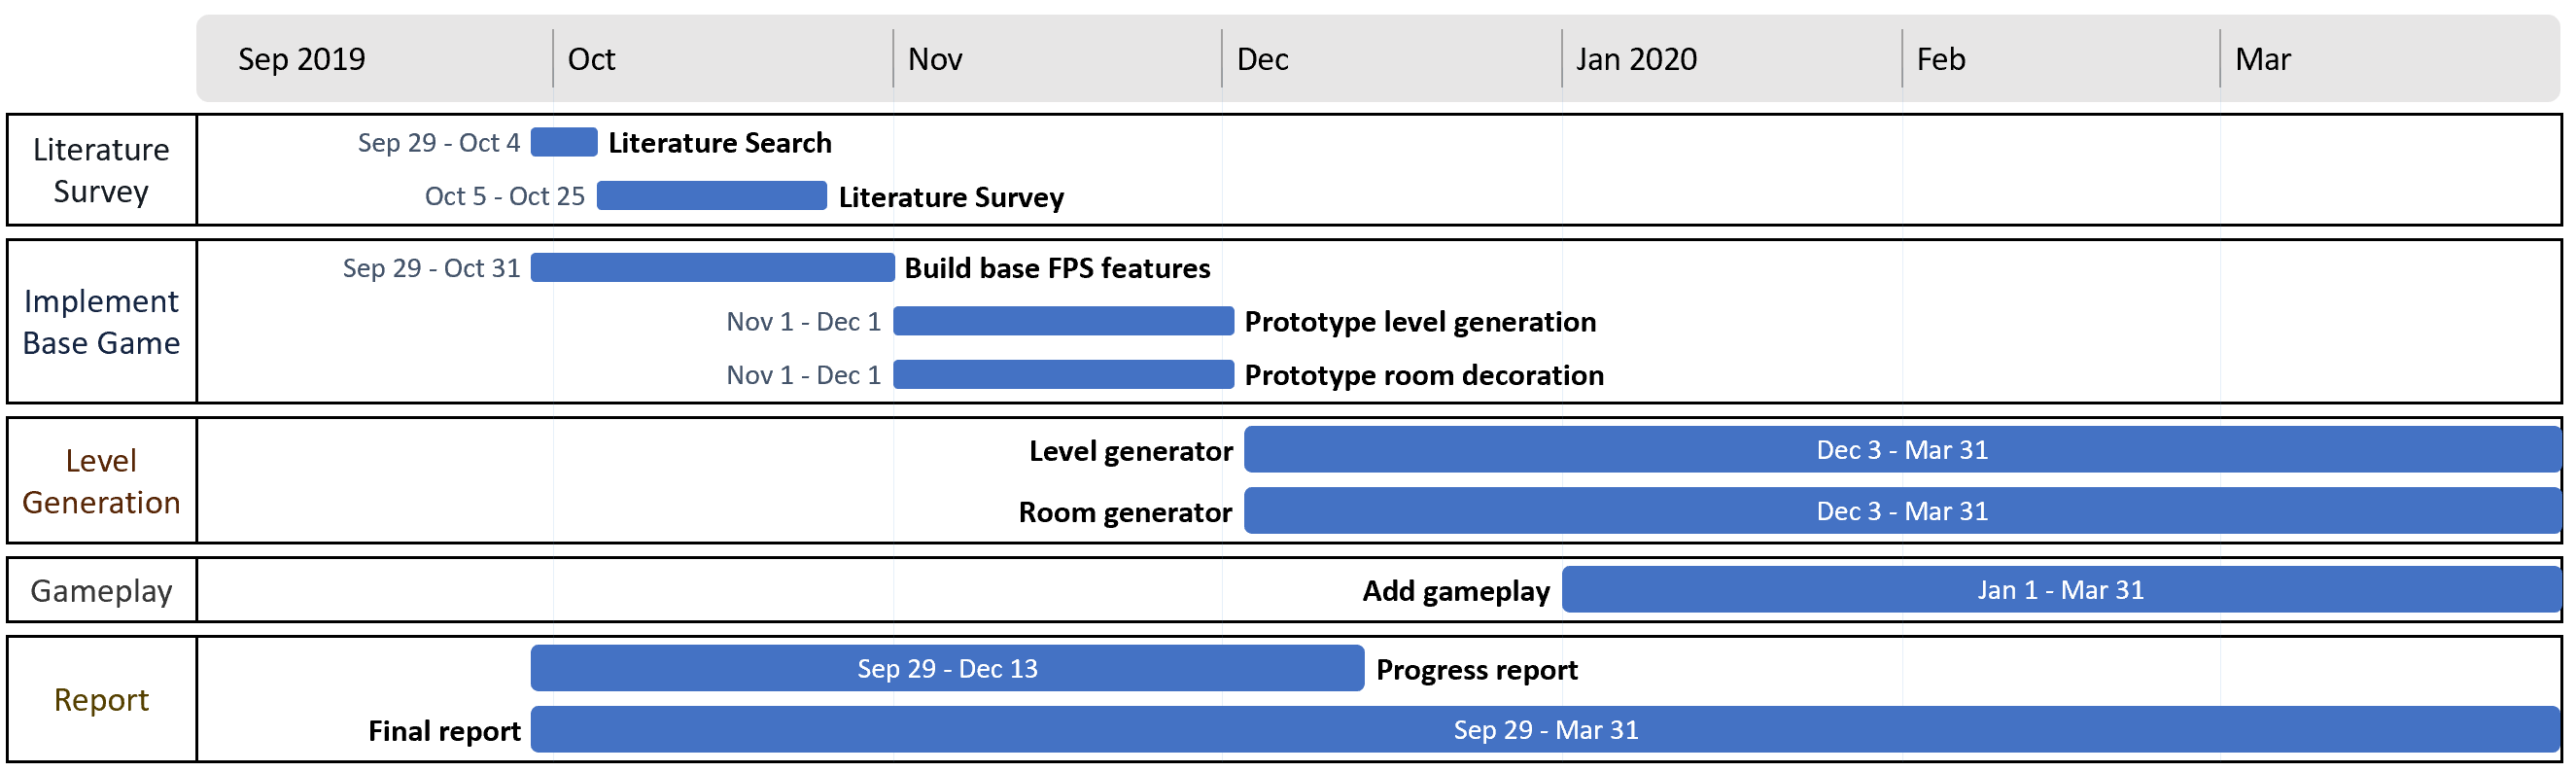
\includegraphics[angle=90,width=\textwidth,height=0.85\textheight,keepaspectratio]{img/gantt-original2.png}
    \caption{Gantt chart of original plan}
    \label{fig:gantt1}
\end{figure}

\begin{figure}[H]
    \centering
    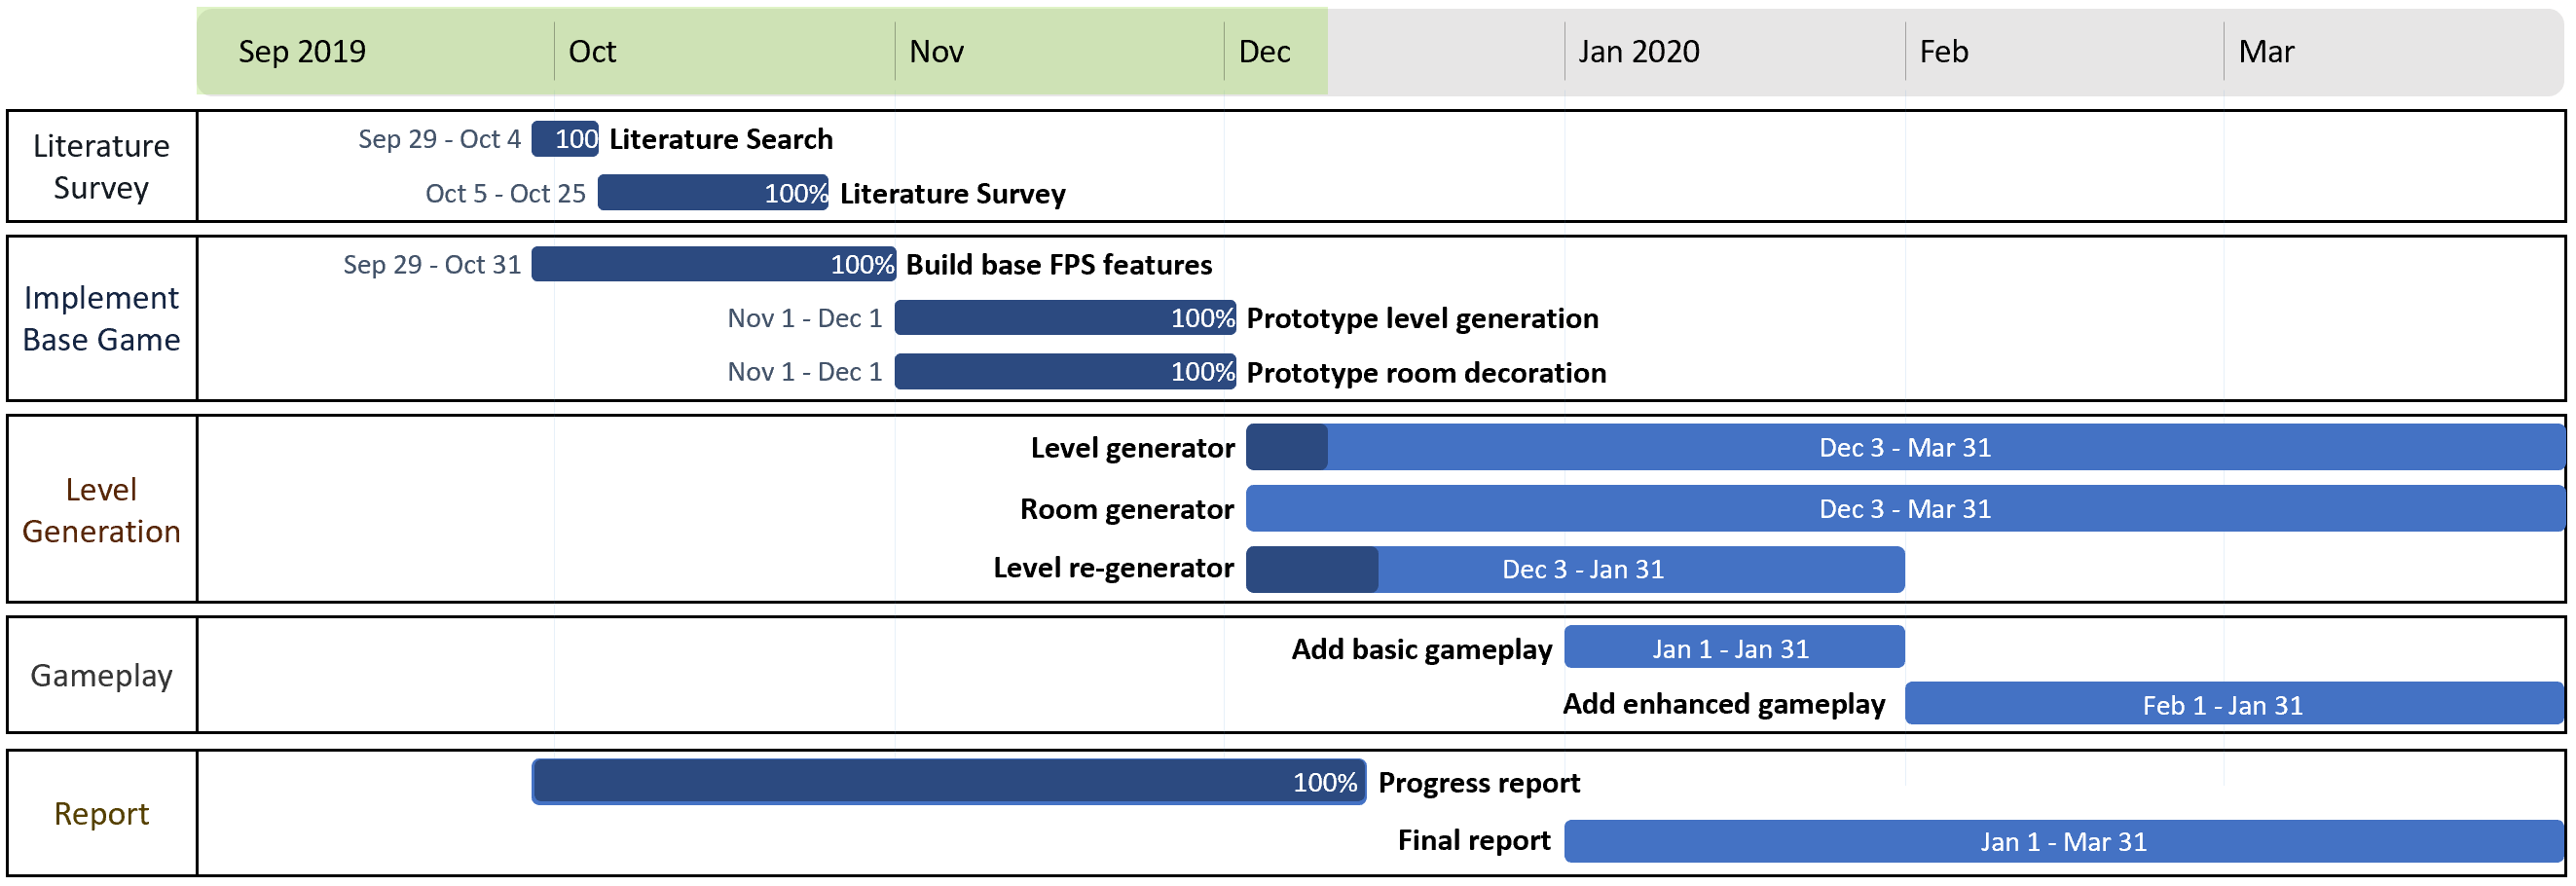
\includegraphics[angle=90,width=\textwidth,height=0.85\textheight,keepaspectratio]{img/gantt-updated2.png}
    \caption{Gantt chart of updated plan}
    \label{fig:gantt2}
\end{figure}

\end{section}

\begin{section}{Diagrams}

\begin{figure}[H]
    \centering
    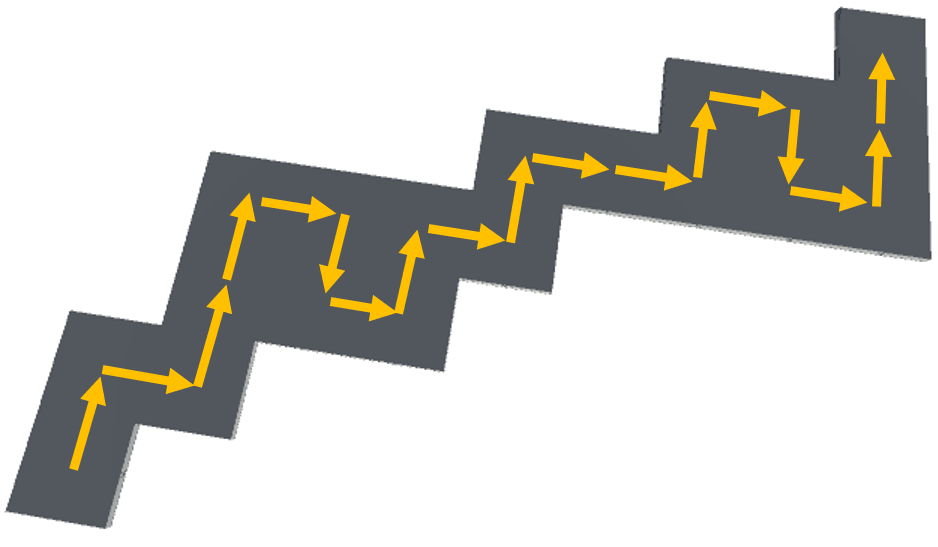
\includegraphics[width=8cm]{img/1-maze.png}
    \caption{A top-down view of the guaranteed path generation, showing how the PCG algorithm moves in three directions to create a route through a maze}
    \label{fig:pathgen}
\end{figure}

\begin{figure}[H]
    \centering
    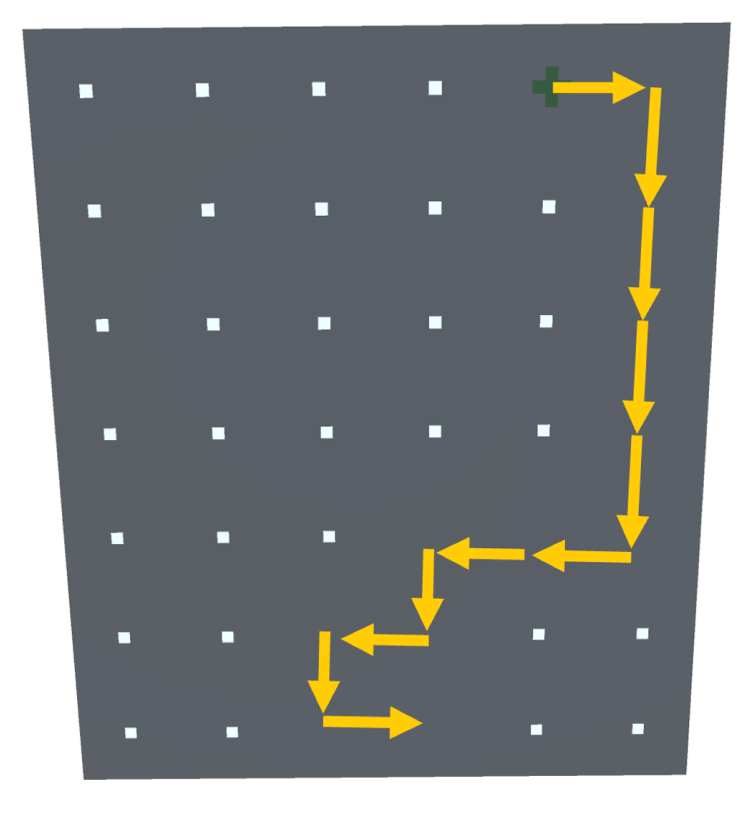
\includegraphics[width=8cm]{img/filled-path.png}
    \caption{A top-down view of the guaranteed path with remaining tiles filled in, demonstrating how the filling algorithm works}
    \label{fig:filledpath}
\end{figure}

\begin{figure}[H]
    \centering
    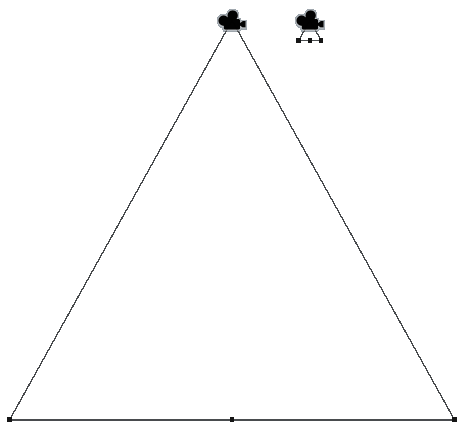
\includegraphics[width=8cm]{img/frustrums.png}
    \caption{A top-down of the difference in default and optimised viewing frustrum sizes, with Unity's default frustrum size on the left and the optimised size for the generated mazes on the right}
    \label{fig:frustrums}
\end{figure}

\begin{figure}[H]
    \centering
    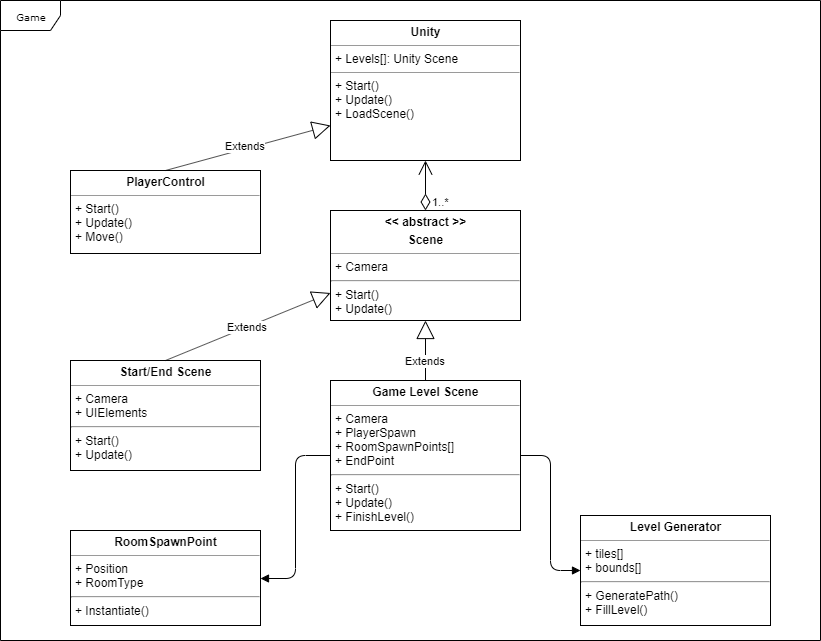
\includegraphics[width=\textwidth]{img/uml1.png}
    \caption{Initial UML diagram}
    \label{fig:uml1}
\end{figure}

\begin{figure}[H]
    \centering
    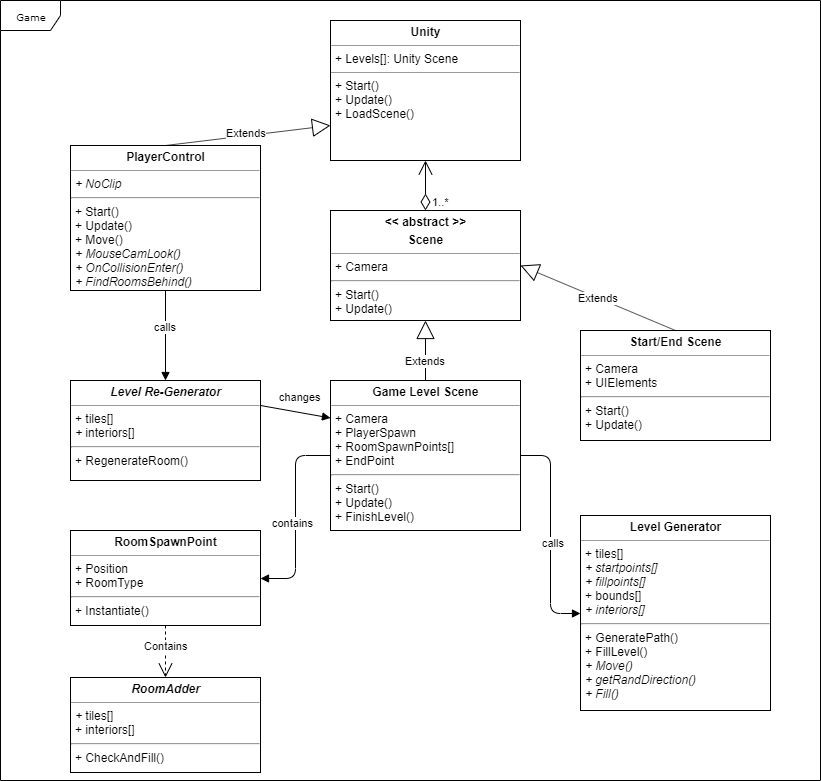
\includegraphics[width=\textwidth]{img/uml2.png}
    \caption{Redesigned UML diagram}
    \label{fig:uml2}
\end{figure}



\end{section}

\begin{section}{Screenshots}
    


\begin{figure}[H]
    \centering
    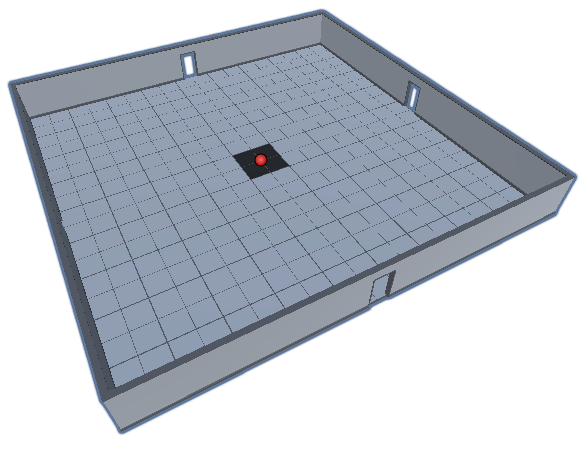
\includegraphics[width=.8\textwidth]{img/prefabroom.png}
    \caption{A screenshot of a room tile, showing the walls and exits of a tile (with the ceiling hidden)}
    \label{fig:prefab-room}
\end{figure}

\begin{figure}[H]
    \centering
    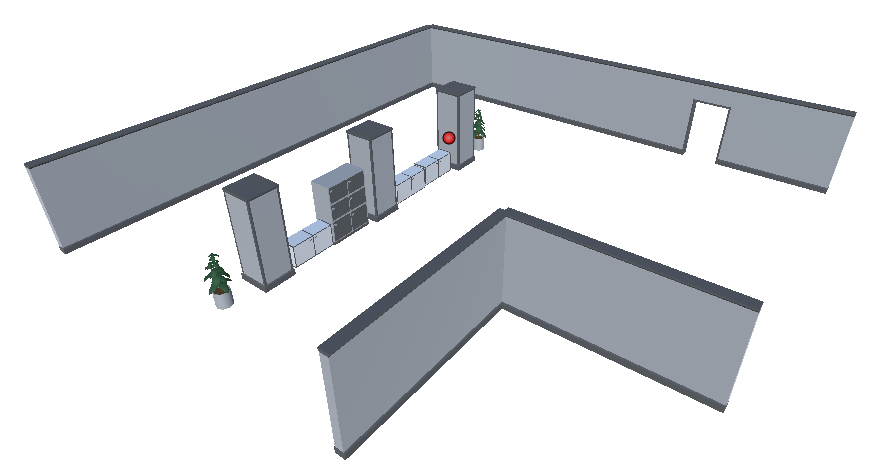
\includegraphics[width=.8\textwidth]{img/interior.png}
    \caption{A screenshot of a room interior, designed to fit into any tile with any exit}
    \label{fig:prefab-int}
\end{figure}

\begin{figure}[H]
    \centering
    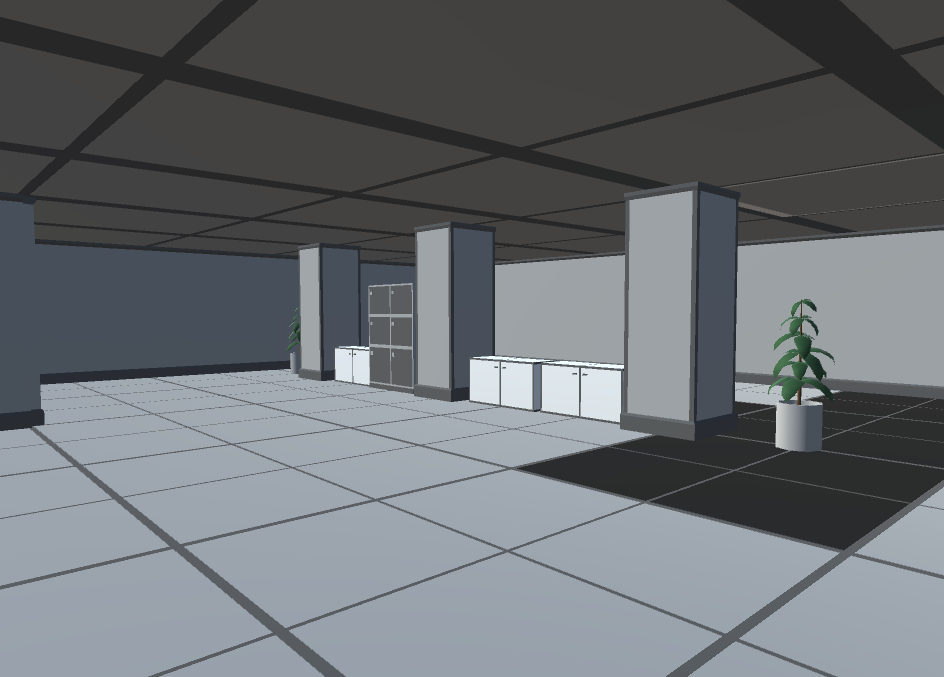
\includegraphics[width=.8\textwidth]{img/imp-int.png}
    \caption{A screenshot of a procedurally generated room, with the tile and interior composited in a real-time environment}
    \label{fig:room}
\end{figure}



\end{section}

\newpage
\begin{section}{Tables}

% epic/story table
\begin{table}[H]
    \resizebox{\textwidth}{!}{%
    \begin{tabular}{@{}ll@{}}
    \toprule
    \multicolumn{1}{l|}{\textbf{Epic}} & \textbf{Stories} \\ \midrule
    \multicolumn{2}{l}{Build base "first person" 3D game features} \\
     & Provides a basic level design \\
     & Proves the concepts of vision and movement \\ \midrule
    \multicolumn{2}{l}{Prototype level generation} \\
     & Prove a method of generating a guaranteed path through a maze \\
     & Prove a method of filling in non-guaranteed paths through the maze \\ \midrule
    \multicolumn{2}{l}{Prototype room generation} \\
     & Prove a method of generating room interiors \\
     & Room generation must not interfere with guaranteed path \\ \midrule
    \multicolumn{2}{l}{Prototype level re-generation} \\
     & Design method to procedurally re-generate level sections \\ \midrule
    \multicolumn{2}{l}{Add gameplay elements} \\
     & Decide on how level is finished by the player \\
     & Provide some interest and threat when playing \\
     & Provide means of assisting navigation \\ \midrule
    \multicolumn{2}{l}{Implement final designs} \\
     & Use non-prototype textures \\
     & Ensure performance meets goals \\ \bottomrule
    \end{tabular}%
    }
    \caption{Agile-style epics and associated user stories}
    \label{tab:epics}
\end{table}

% Please add the following required packages to your document preamble:
% \usepackage{graphicx}
\begin{table}[H]
    \resizebox{\textwidth}{!}{%
    \begin{tabular}{llll}
    \hline
    \multicolumn{1}{|l|}{\textbf{Requirement type}} & \multicolumn{1}{l|}{\textbf{Requirement}} & \multicolumn{1}{l|}{\textbf{Priority}} & \multicolumn{1}{l|}{\textbf{Status}} \\ \hline
    Epic & Write Project Proposal & Should Have & Done \\
    - Requirement & Research PCG & Should Have & Done \\
    - Requirement & Write proposal & Should Have & Done \\ \hline
    Epic & Write Literature Review & Should Have & Done \\
    - Requirement & Research/find literature & Should Have & Done \\
    - Requirement & Get feedback & Should Have & Done \\
    - Requirement & Write review & Should Have & Done \\ \hline
    Epic & Build base FPS features & Must Have & Done \\
    - Requirement & Create title/game over screens & Should Have & Done \\
    - Requirement & Create end goal, transitions to end screens & Should Have & Done \\
    - Requirement & Implement first person controller & Must Have & Done \\ \hline
    Epic & Prototype level generation & Must Have & Done \\
    - Requirement & Design room tile prefabs & Must Have & Done \\
    - Requirement & Implement "random walk" generation & Must Have & Done \\
    - Requirement & Implement maze filling algorithm & Must Have & Done \\
    - Requirement & Implement different sized tiles & Could Have &  \\ \hline
    Epic & Prototype room decoration & Must Have & Done \\
    - Requirement & Design room decoration prefabs & Must Have & Done \\
    - Requirement & Implement room decoration filling algorithm & Must Have & Done \\
    - Requirement & Design random sub-decorator agents & Could Have & Done \\ \hline
    Epic & Progress report & Must Have & Done \\
    - Requirement & Design plan & Should Have & Done \\
    - Requirement & Write first draft & Should Have & Done \\
    - Requirement & Write final draft and submit & Must Have &  \\ \hline
    Epic & Prototype re-generation & Must Have &  \\
    - Requirement & Design approach for re-generating parts of level in real-time & Must Have &  \\
    - Requirement & Implement re-generation process & Must Have &  \\
    - Requirement & Implement re-generation trigger process & Must Have &  \\ \hline
    Epic & Level generator & Must Have &  \\ \hline
    Epic & Room generator & Must Have &  \\ \hline
    Epic & Level re-generator & Must Have &  \\ \hline
    Epic & Basic gameplay & Must Have &  \\ \hline
    Epic & Enhanced gameplay & Should Have &  \\ \hline
    Epic & Final report & Must Have &  \\ \hline
    \end{tabular}%
    }
    \caption{A table showing epics and requirements, their priorities and statuses}
    \label{tab:epicreqs}
\end{table}


\end{section}

\end{document}
